Pizzinelli et al.\ (\citeyear{Pizzinelli2023Labor}) extend the AIOE framework with a \textit{complementarity index} that measures how much AI supports rather than substitutes human labor. The index uses 11 O*NET work context variables (scored 0--100 by importance or frequency) and Job Zone (ordinal 1--5, rescaled to 0--100), grouped into six dimensions:
\begin{enumerate}
    \item \textbf{Communication} -- Face-to-Face Discussions, Public Speaking;
    \item \textbf{Responsibility} -- Responsibility for Outcomes, Responsibility for Others’ Health;
    \item \textbf{Physical Conditions} -- Outdoor Environments, Physical Proximity;
    \item \textbf{Criticality} -- Consequence of Errors, Freedom of Decisions, Frequency of Decisions;
    \item \textbf{Routine} -- Degree of Automation (inverted to ``Degree of Freedom'')\footnote{The inversion is defined as $\text{Degree of Freedom} = 100 - \text{Degree of Automation}.$ This ensures that higher Degree of Freedom values reflect greater AI complementarity.}, Structured vs.\ Unstructured Work; and
    \item \textbf{Skills} -- Job Zone (scaled from 1 = least preparation to 5 = most preparation).
\end{enumerate}
Each dimension score is the mean of its components, and the overall index is the mean across all six. To interpret complementarity, as the score of any dimension increases, AI is more likely to augment labor, and thus the complementarity index also increases.

To verify the consistency of our methodology, we compared the correlation matrix of the six computed dimensions with the corresponding matrix reported in the study. 
Since the pairwise correlations in our results closely align with those presented by Pizzinelli et al. as shown in Figure~\ref{fig:correl_heatmaps}, we can reasonably conclude that our implementation of the methodology is correct.
\begin{figure}[ht] 
    \centering 
    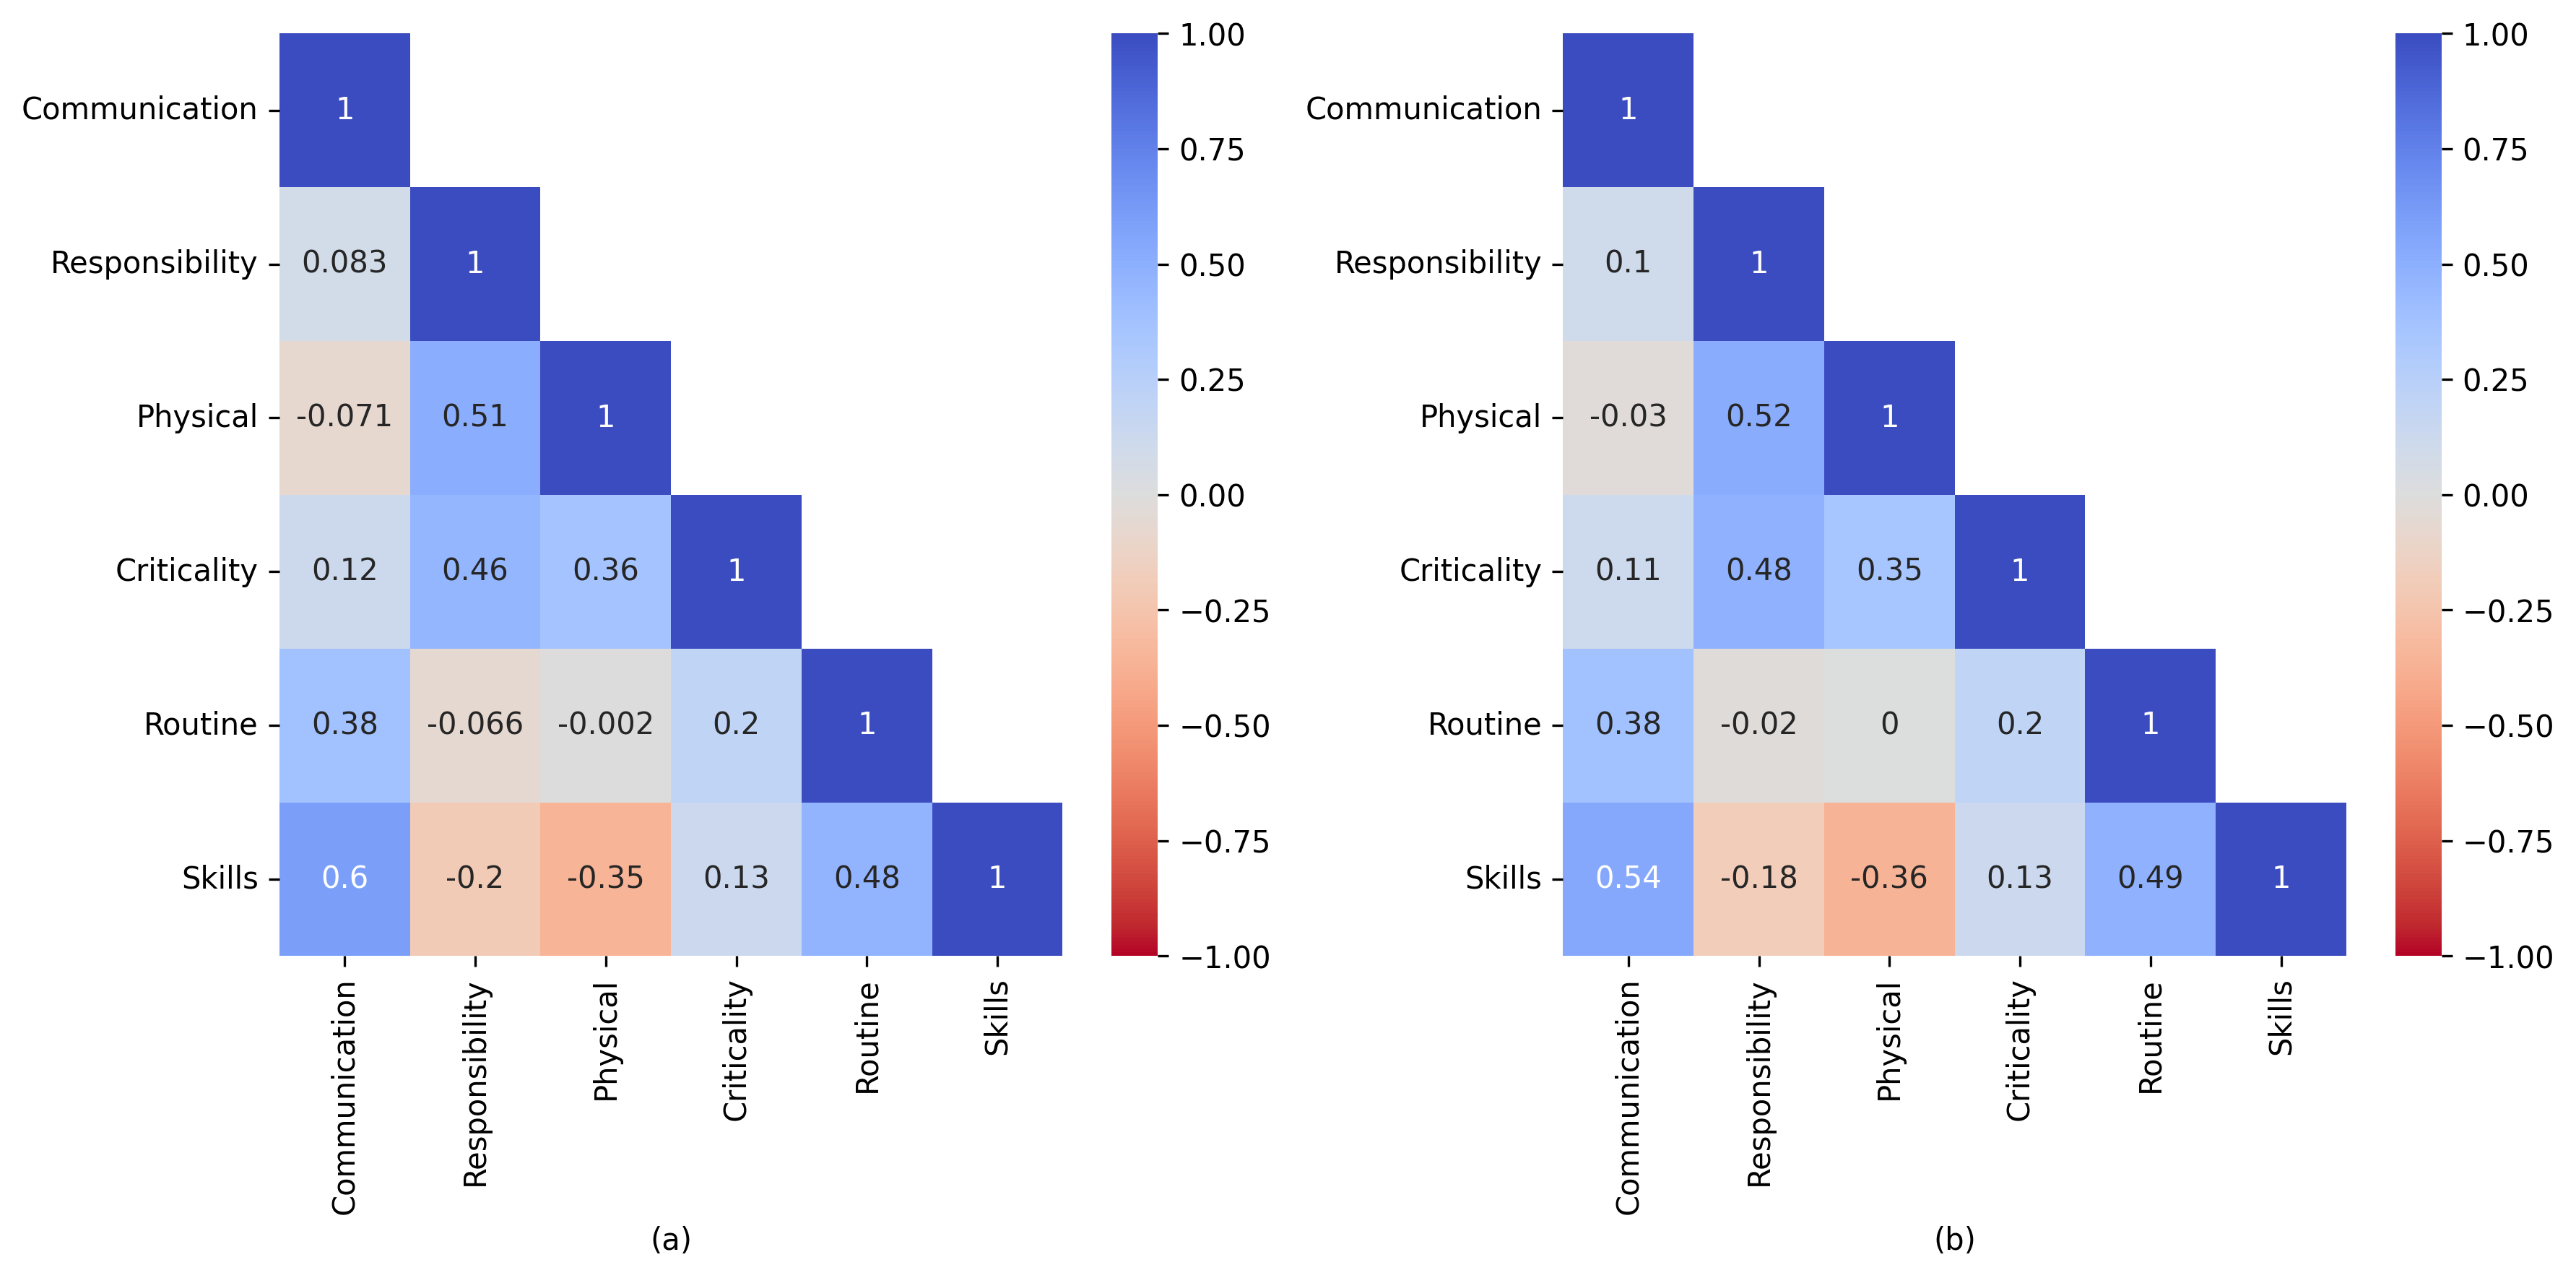
\includegraphics[width=\linewidth]{../figures/correls.png} 
    \caption{Correlation Matrices by Pizzinelli et al. (a) and by Viray and Oximas (b)} 
    \label{fig:correl_heatmaps} 
\end{figure}

Similar to assigning the AIOE, some SOC codes did not get a complementarity score because of legacy classifications. Even after accounting for legacy codes, roughly 16.9\% of jobs lacked complementarity scores, which we imputed using the mean score of their major-minor SOC group.